\documentclass[twocolumn,10pt]{article}
\usepackage[a4paper,margin=1.8cm,top=2cm,bottom=2cm]{geometry}
\usepackage{amsmath,amssymb,graphicx,booktabs,xcolor}
\usepackage[colorlinks=true,linkcolor=blue!60!black,citecolor=blue!60!black,urlcolor=blue!60!black]{hyperref}
\usepackage{microtype}
\usepackage[authoryear,round]{natbib}
\graphicspath{{figures/}}
\setlength{\parskip}{2pt}
\newcommand{\LX}{L_{\mathrm{X}}}
\newcommand{\LUV}{L_{\mathrm{UV}}}
\newcommand{\FX}{F_{\mathrm{X}}}
\newcommand{\FUV}{F_{\mathrm{UV}}}
\newcommand{\DL}{D_{\mathrm{L}}}

\title{\Large\bf Is a flat $\gamma(z)$ enough? Redshift, luminosity and selection\\
degeneracies in the quasar $\LX$--$\LUV$ slope, and what they cost the Hubble diagram}
\author{Nasser Abu Seif$^{1}$ and Abdel-Rahman Nasser$^{2}$\\[3pt]
\small $^{1}$National Research Institute of Astronomy and Geophysics (NRIAG), Helwan, Cairo, Egypt\\
\small $^{2}$Independent researcher, Phoenix, AZ, USA}
\date{\small Draft v1 --- 3 September 2026. Code, data and every quoted number: \url{https://github.com/AbdelRahmanNasser20/quasar-standard-candles}}

\begin{document}
\maketitle

\begin{abstract}
\noindent
Quasars can serve as standardizable candles only if the slope $\gamma$ of the $\log\LX=\gamma\log\LUV+\beta$ relation does not change with cosmic time. The standard test fits $\gamma$ in narrow redshift bins and asks whether it is flat. We point out that in flux-limited samples this test is under-determined: in the public Lusso et al.\ (2020) catalogue of 2421 quasars, the bin-mean UV luminosity and the bin redshift are collinear at $r=0.98$ ($d\langle\log\LUV\rangle/dz=0.67$\,dex), so a redshift-dependent slope $\gamma(z)$ and a luminosity-dependent slope $\gamma(\LUV)$ fit the binned slopes equally well ($\Delta{\mathrm{AIC}}=1.1$). We introduce a binning-free, cosmology-free joint likelihood in flux--flux space with one distance nuisance parameter per narrow redshift shell and a global $\gamma(z)=\gamma_0+m(z-1.3)$, and obtain $\gamma_0=0.582\pm0.011$, $\delta=0.225$\,dex and $m=-0.042^{+0.016}_{-0.017}$ (likelihood-ratio $p=0.007$; BIC does not prefer the extra parameter). We then test, one by one, the non-cosmological explanations. (i) Luminosity curvature: the cosmology-free within-shell curvature $d\gamma/d\log\LUV=+0.042\pm0.028$ has the wrong sign and is $3.7\sigma$ away from the $-0.062$ needed to mimic the drift. (ii) Flux-limit truncation: a truncated-Gaussian likelihood shifts individual slopes by $+0.007$ to $+0.04$ but leaves $m$ unchanged. (iii) X-ray photon index: a $\Gamma_{\mathrm{X}}$ term lowers the intrinsic scatter from 0.224 to 0.211\,dex ($-0.33\pm0.02$\,dex per unit $\Gamma_{\mathrm{X}}$) and leaves $m$ negative. (iv) Within-shell distance variation: detrending fluxes to the shell-centre distance changes $m$ by $<0.001$. (v) Sample heterogeneity: the homogeneous SDSS--4XMM subsample alone gives $m=-0.060\pm0.021$. The drift is, however, carried by the $z<0.7$ shells: above $z=0.7$, $m=-0.022\pm0.019$, consistent with zero and with the new homogeneous sample of Risaliti et al.\ (2026). Finally we translate the allowed drift into a distance error: at $z=2$ the best-fit drift corresponds to $\Delta\mu=-0.56$\,mag (23\% in $\DL$) and the $2\sigma$ bound to 0.9\,mag; a 2\% distance at $z=2$ requires $\sigma_m\simeq0.003$, about 25 times more quasars than the present catalogue, or an external anchor at every redshift. A flat $\gamma(z)$ measured to $\pm0.02$ is therefore a necessary but far from sufficient condition for quasar cosmology.
\end{abstract}

\section{Introduction}
The non-linear relation between the ultraviolet and X-ray luminosities of quasars, $\log\LX=\gamma\log\LUV+\beta$ with $\gamma\simeq0.6$, has been known since the \textit{Einstein} era \citep{tananbaum79,avni86} and is understood as the imprint of the coupling between the accretion disc and the Comptonizing corona \citep{haardt91,lusso17,kubota18}. Risaliti \& Lusso (2015, 2019) and Lusso et al.\ (2020, hereafter L20) turned it into a distance indicator: if $\gamma$ and $\beta$ are universal, the observed fluxes of a quasar give its luminosity distance,
\begin{equation}
\log\DL=\frac{\log\FX-\gamma\log\FUV-\beta'}{2(\gamma-1)},\qquad \beta'=\beta+(\gamma-1)\log4\pi ,
\label{eq:dl}
\end{equation}
and a Hubble diagram can be built out to $z\simeq7$, where Type Ia supernovae are unavailable. The stakes are the $5\sigma$ Hubble tension between the local ladder \citep{riess22} and the CMB \citep{planck20}; see \citet{divalentino21} for a review.

The method has a single load-bearing assumption: $\gamma$ must not depend on redshift. The community tests this by fitting the relation in narrow redshift bins in flux--flux space, where the distance is approximately common to all objects in the bin and cosmology drops out, and checking that the bin slopes are flat. On this test the literature is split. L20, the eROSITA analysis of \citet{sacchi25}, and the new homogeneous sample of \citet{risaliti26} find a flat slope, $\gamma\simeq0.58$--$0.60$. \citet{khadka20,khadka21,khadka22} find that the L20 compilation is not standardizable above $z\simeq1.5$--$1.7$; \citet{dainotti22}, \citet{lenart23} and \citet{dainotti23} detect and correct a $(1+z)^k$ evolution of both luminosities with the Efron--Petrosian method; \citet{wang22,wang24} favour a copula-based redshift-evolutionary relation at $>3\sigma$; \citet{li25} find a $4\sigma$ high/low-redshift inconsistency when the relation is calibrated on supernovae; \citet{li26} find simultaneous dependence on redshift and X-ray photon index; and \citet{gao26} find that even the intrinsic scatter is redshift dependent above $z\simeq1.6$. \citet{petrosian22} argue on general grounds that a luminosity--luminosity correlation cannot by itself fix the distance--redshift relation, and \citet{lusso25} concede deviations from $\Lambda$CDM above $z\simeq1.5$ while excluding severe systematics in the data.

This paper does not take a side. It makes three narrower points on the public L20 catalogue.
\begin{enumerate}\setlength{\itemsep}{0pt}
\item In a flux-limited sample redshift and luminosity are collinear, so ``$\gamma(z)$ is flat'' and ``$\gamma(\LUV)$ is flat'' are the same statement to the binned test. We quantify the collinearity and show which additional, cosmology-free measurement breaks it (Section~\ref{sec:degeneracy}).
\item We measure the redshift drift of $\gamma$ with a binning-free joint likelihood and then attack it with every non-cosmological explanation we can test on the catalogue itself (Sections~\ref{sec:joint}--\ref{sec:doubt}).
\item We convert the allowed drift into the distance error it produces and into the precision on $m=d\gamma/dz$ that a percent-level $H_0$ from quasars alone would require (Section~\ref{sec:cost}).
\end{enumerate}
An earlier draft by one of us (N.\,A.\,S., 2026, unpublished) reported $m=-0.002\pm0.007$ on this catalogue. That value does not reproduce and the present analysis supersedes it; the audit is in the companion folder of our repository.

\section{Data}
\label{sec:data}
We use table~3 of L20 exactly as distributed by CDS/VizieR (\texttt{J/A+A/642/A150}): 2421 quasars with rest-frame $2500$\,\AA\ and 2\,keV monochromatic fluxes, their errors, the X-ray photon index $\Gamma_{\mathrm{X}}$, and a group flag identifying the sub-sample each object comes from. Redshifts span $0.009\le z\le7.54$ with median 1.30. L20 already removed broad-absorption-line and radio-loud objects, dust-reddened sources ($E(B-V)>0.1$), X-ray absorbed sources ($\Gamma_{\mathrm{X}}$ outside 1.7--2.8) and objects liable to Eddington bias. We apply no further cut. Group~5, the SDSS-DR14Q\,$\times$\,4XMM-DR9 cross-match, holds 1644 objects; group~6 (608) is the Chandra sample; groups 1--4 and 7 (169 objects) are small local and high-redshift additions. Luminosities are used only (a) to define the luminosity axis of Fig.~\ref{fig:coll}, (b) for the full-sample curvature test of Section~\ref{sec:curv}, and (c) to define the anchor in Section~\ref{sec:cost}; for these we adopt a flat $\Lambda$CDM with $H_0=70$\,km\,s$^{-1}$\,Mpc$^{-1}$ and $\Omega_m=0.315$ and verify insensitivity to $\Omega_m\in[0.25,0.40]$. The full-sample luminosity-space fit reproduces the well-known values $\gamma=0.664\pm0.007$, $\beta=6.33\pm0.22$, $\delta=0.230\pm0.004$\,dex; we do not use them further because they are the cosmology-dependent quantities the flux--flux method is designed to avoid.

\section{The redshift--luminosity degeneracy}
\label{sec:degeneracy}
We divide the sample into shells of width $\Delta\log(1+z)=0.03$ and keep the 18 shells with at least 25 objects (2336 quasars, $0.29\le\langle z\rangle\le3.14$). Figure~\ref{fig:coll} shows the shell-mean $\log\LUV$ against the shell-mean redshift: the two are collinear with correlation coefficient $r=0.982$ and slope $0.67$\,dex per unit redshift. Any smooth dependence of the slope on redshift, $\gamma=\gamma_0+m\,(z-1.3)$, is therefore observationally equivalent to a dependence on luminosity, $\gamma=\gamma_0+\kappa\,(\langle\log\LUV\rangle-30)$, with $\kappa\simeq m/0.67$.

\begin{figure}
\centering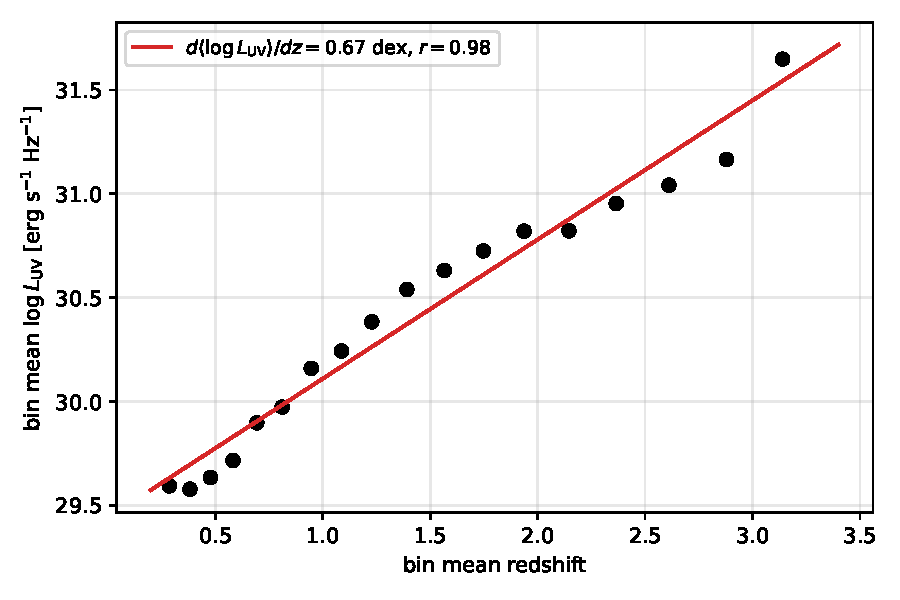
\includegraphics[width=\columnwidth]{fig2_collinearity}
\caption{Shell-mean UV luminosity against shell-mean redshift for the 18 narrow shells. The collinearity ($r=0.98$) is a property of any flux-limited sample and is what makes ``$\gamma$ is flat in $z$'' and ``$\gamma$ is flat in $\LUV$'' indistinguishable to a binned test.}
\label{fig:coll}
\end{figure}

We make this explicit with a joint likelihood. For quasar $i$ in shell $s(i)$ let $u_i=\log F_{\mathrm{UV},i}-\tilde x_{s(i)}$ be the UV flux offset from the median of its own shell. We model
\begin{equation}
\log F_{\mathrm{X},i}=\gamma_i\,u_i+\beta_{s(i)},\qquad
\gamma_i=\begin{cases}\gamma_0 & \text{(C)}\\ \gamma_0+m\,(z_i-1.3) & \text{(Z)}\\ \gamma_0+\kappa\,(\langle\log\LUV\rangle_{s(i)}-30) & \text{(L)}\end{cases}
\end{equation}
with one free intercept $\beta_s$ per shell, which absorbs the (unknown) luminosity distance of that shell, and a single intrinsic scatter $\delta$. The likelihood is that of \citet{dagostini05}, with variance $\delta^2+\sigma_{y,i}^2+\gamma_i^2\sigma_{x,i}^2$. Model C has $2+18$ parameters, models Z and L have $3+18$. No cosmology enters models C and Z at all; model L uses the fiducial cosmology only to order the shells along the luminosity axis.

Table~\ref{tab:models} gives the result. Models Z and L are indistinguishable ($\Delta{\mathrm{AIC}}=1.1$). Both improve on the constant slope by $2\Delta\ln\mathcal L=7.3$ ($p=0.007$ for one extra parameter); the BIC, with its stronger penalty, prefers the constant slope by 0.4. The evidence for any drift is thus moderate, and the evidence for its being a \emph{redshift} drift rather than a \emph{luminosity} drift is nil, as it must be given Fig.~\ref{fig:coll}.

\begin{table}
\centering\small
\caption{Joint flux--flux fits with 18 shell intercepts (2336 quasars). $\gamma_0$ is the slope at $z=1.3$ (models C, Z) or at $\log\LUV=30$ (model L).}
\label{tab:models}
\begin{tabular}{lccccc}
\toprule
Model & $\gamma_0$ & slope param. & $\delta$ & AIC & BIC\\
\midrule
C: constant & 0.578 & --- & 0.224 & $-147.96$ & $-32.84$\\
Z: $\gamma(z)$ & 0.583 & $m=-0.044$ & 0.224 & $-153.28$ & $-32.40$\\
L: $\gamma(\LUV)$ & 0.608 & $\kappa=-0.069$ & 0.224 & $-154.34$ & $-33.46$\\
\bottomrule
\end{tabular}
\end{table}

\section{The drift and its uncertainty}
\label{sec:joint}
Sampling model Z with \textsc{emcee} \citep{foremanmackey13} (46 walkers, 4000 steps, 1500 discarded; the 18 intercepts marginalised) gives
\begin{equation}
\gamma_0(z{=}1.3)=0.582\pm0.011,\quad m=-0.042^{+0.016}_{-0.017},\quad \delta=0.225\,{\mathrm{dex}},
\end{equation}
with $P(m\ge0)=0.3\%$ and a 95\% bound $|m|<0.070$. A rerun with a different random seed gives $m=-0.046\pm0.017$. Figure~\ref{fig:gz} shows the per-shell slopes (plain fits, bootstrap errors) with the joint fit overlaid. The per-shell errors are 0.03--0.05 for 150--330 objects, so any four-bin estimate of $m$ on this catalogue has $\sigma_m\gtrsim0.013$; claims of $\sigma_m<0.01$ from these data are not achievable.

\begin{figure}
\centering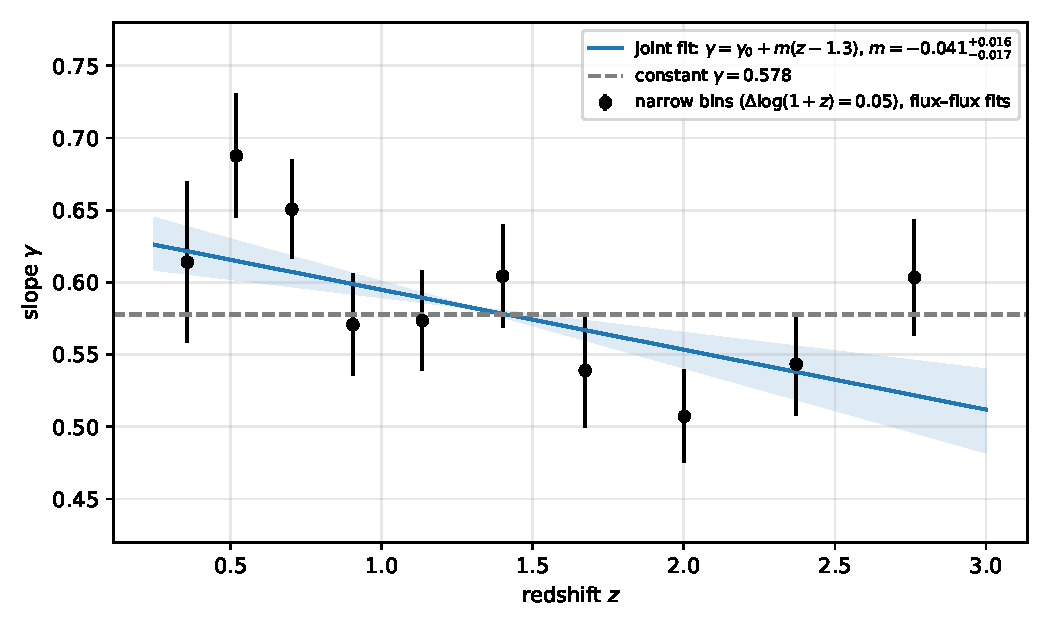
\includegraphics[width=\columnwidth]{fig1_gamma_z}
\caption{Slope $\gamma$ in narrow flux--flux shells ($\Delta\log(1+z)=0.05$ here for legibility; the joint fit uses 0.03). Blue: model Z with its 68\% band. Grey: the constant-slope fit. The drift is carried by the shells below $z\simeq0.7$.}
\label{fig:gz}
\end{figure}

The drift's \emph{sign} is stable against the shell width: for $\Delta\log(1+z)=0.03, 0.04, 0.05, 0.07, 0.10$ the binned estimates are $m=-0.056, -0.036, -0.043, -0.070, -0.065$ with errors 0.015--0.019. Its \emph{significance} is not: the $\chi^2$ of a constant slope has $p$ between 0.026 and $<0.001$ depending on the binning, which is why we quote the binning-free value above.

\section{Doubting the drift}
\label{sec:doubt}
We now try to remove the drift with every non-cosmological mechanism the catalogue lets us test. Table~\ref{tab:robust} summarises.

\subsection{Luminosity curvature}
\label{sec:curv}
If the true relation is curved, $\log\LX=\gamma_0 u+q u^2+\beta$, the local slope is $d\gamma/d\log\LUV=2q$ and the drift in Table~\ref{tab:models} would be a luminosity effect masquerading as evolution. Model L requires $\kappa=m/0.67=-0.062$. The curvature can be measured \emph{within} each shell, cosmology-free, because inside a shell luminosity and flux differ by a constant. Fitting the quadratic in the 12 shells with $N\ge100$ (bootstrap errors) gives a weighted $q=+0.021\pm0.014$, i.e.\ $2q=+0.042\pm0.028$ (Fig.~\ref{fig:curv}): the wrong sign, and $3.7\sigma$ from the value required. The full-sample luminosity-space quadratic, which does depend on cosmology, gives $q=-0.008\pm0.007$ for $\Omega_m=0.25, 0.315, 0.40$, also inconsistent with $q=-0.031$. Luminosity curvature does not explain the drift. (Flux-limit truncation flattens the faint end and would bias $q$ positive; this makes the test conservative in the direction of rejecting curvature, but a truncation-aware curvature fit is beyond the present data.)

\begin{figure}
\centering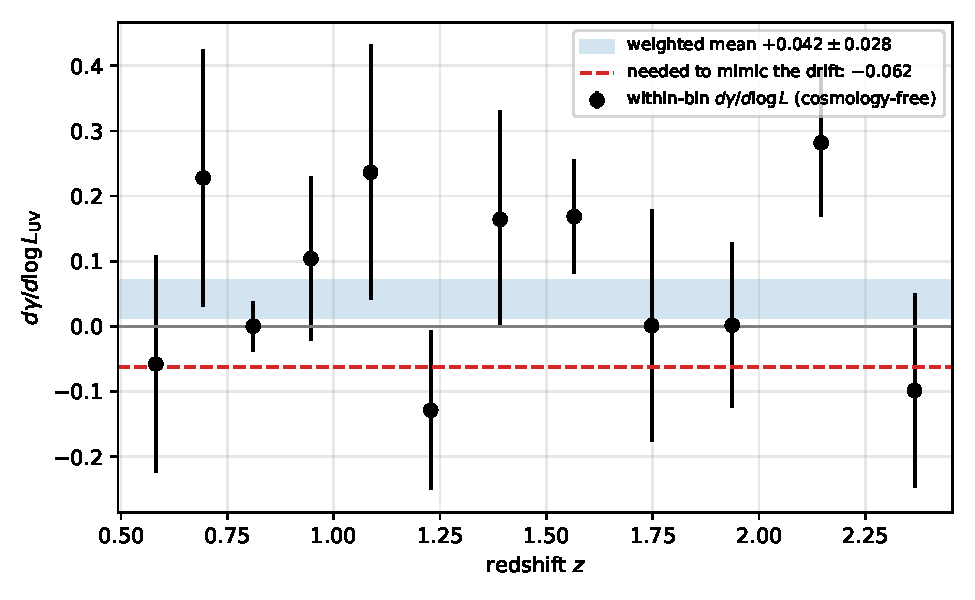
\includegraphics[width=\columnwidth]{fig3_curvature}
\caption{Within-shell slope curvature $d\gamma/d\log\LUV=2q$ (cosmology-free), its weighted mean (band), and the value a luminosity-dependent slope would need in order to mimic the observed redshift drift (dashed).}
\label{fig:curv}
\end{figure}

\subsection{Flux-limit truncation}
At high redshift only the X-ray brightest objects at a given UV flux survive the detection limit; this cuts the faint end of the dependent variable and flattens the slope, mimicking a negative $m$ \citep{eddington13,kelly07}. In the catalogue, 22\% of the lowest shell and 13--26\% of the two highest shells lie within 0.3\,dex of the shell's faintest X-ray flux, so the limit does bite at both ends. We refit each shell with a truncated-Gaussian likelihood, $p(y\,|\,x,\,y>y_{\mathrm{lim}})=\mathcal N(y;\mu,s)/[1-\Phi((y_{\mathrm{lim}}-\mu)/s)]$, taking $y_{\mathrm{lim}}$ at the 0th, 1st or 3rd percentile of the shell's $\log\FX$. The correction raises the individual slopes by $+0.007$, $+0.022$, $+0.043$ on average for the three floors, but the fitted drift is unchanged: $m=-0.056, -0.040, -0.059$ versus $-0.053, -0.033, -0.047$ uncorrected, all $\pm0.02$ (Fig.~\ref{fig:trunc}). A sharp floor is a crude model of the SDSS\,$\times$\,XMM selection, so this excludes only the simplest form of truncation bias; a forward model of the survey selection function \citep[as in][]{signorini24} remains the definitive test.

\begin{figure}
\centering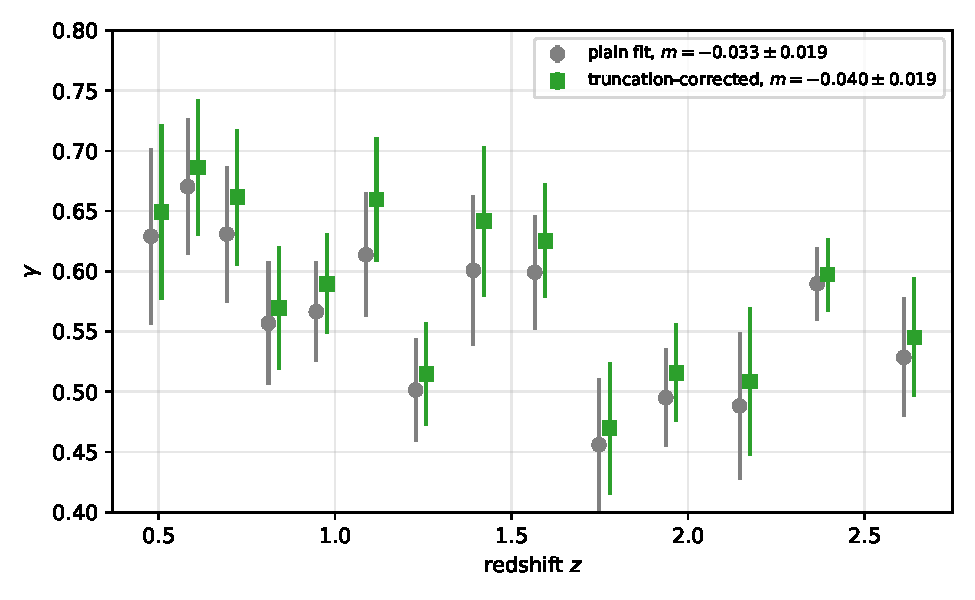
\includegraphics[width=\columnwidth]{fig4_truncation}
\caption{Per-shell slopes with a plain likelihood (grey) and a truncated-Gaussian likelihood with the floor at the shell's 1st percentile in $\log\FX$ (green, offset in $z$ for clarity). The correction shifts the slopes up but not the drift.}
\label{fig:trunc}
\end{figure}

\subsection{X-ray photon index}
Both $\Gamma_{\mathrm{X}}$ and redshift are available per object. $\Gamma_{\mathrm{X}}$ correlates weakly with redshift (Spearman $\rho=0.14$, $p=10^{-12}$) and, within shells, hardly at all with UV flux ($\langle r\rangle=-0.05$). Adding a term $c\,(\Gamma_{\mathrm{X}}-2.175)$ to model Z gives $c=-0.33\pm0.02$\,dex per unit photon index and lowers $\delta$ from 0.224 to 0.211\,dex, while $m=-0.063\pm0.015$ stays negative. We do not interpret $c$ physically: the rest-frame 2\,keV flux in L20 is derived from band fluxes using $\Gamma_{\mathrm{X}}$, so part of $c$ is methodological. Splitting the sample at the median $\Gamma_{\mathrm{X}}$ gives $m=-0.052\pm0.021$ (soft half) and $-0.065\pm0.022$ (hard half). The photon-index mix does not create the drift; see \citet{li26} for a fuller treatment.

\subsection{Within-shell distance variation}
Even in a shell of $\Delta\log(1+z)=0.03$ the luminosity distance varies, coherently moving objects along a slope-1 line and biasing $\gamma$ towards unity, most strongly at low redshift. The standard deviation of $2\log\DL$ within a shell falls from 0.095\,dex at $\langle z\rangle=0.29$ to 0.03\,dex at $z>1.9$. We remove the effect by rescaling each object's fluxes to the shell-median distance, $F'=F\,(\DL(z)/\DL(z_{\mathrm{shell}}))^2$, which uses only the shape of $\DL(z)$ inside the shell ($H_0$ cancels). The result is $m=-0.046\pm0.016$, $-0.043\pm0.016$, $-0.043\pm0.016$ for $\Omega_m=0.315, 0.25, 0.40$, against $-0.046\pm0.017$ undetrended. The effect is real in principle but too small to matter here.

\subsection{Sample heterogeneity and redshift range}
The homogeneous group~5 (SDSS\,$\times$\,4XMM, 1619 objects in the shells) gives $m=-0.060\pm0.021$, $P(m\ge0)=0.2\%$; groups 5+6 give $-0.041\pm0.017$. Heterogeneity does not create the drift either.

What does matter is the redshift range. Restricting to $z>0.7$, the range of the new homogeneous sample of \citet{risaliti26}, gives $m=-0.022\pm0.019$ ($P(m\ge0)=13\%$), fully consistent with zero and with their $\gamma=0.58\pm0.01$; group~5 above $z=0.7$ gives $-0.049\pm0.027$. The shells below $z=0.7$ alone (364 objects) cannot constrain a slope ($\gamma_0=0.85\pm0.18$) but have individually high slopes, 0.61--0.69. The drift in the L20 compilation is therefore a statement about the contrast between $z<0.7$ and $z>0.7$, not a smooth trend across $0.7<z<3$. This reconciles, at least on this catalogue, the ``no evolution'' results of L20, \citet{sacchi25} and \citet{risaliti26}, all of which start at or above $z\simeq0.7$ or concern eROSITA depths, with the high/low-redshift inconsistencies of \citet{khadka21} and \citet{li25}, whose low-redshift anchors reach down to $z\simeq0.1$. We cannot say from these data whether the low-redshift excess in $\gamma$ is astrophysical (host-galaxy light at 2500\,\AA\ would raise $\FUV$ preferentially for faint, low-$z$ objects and steepen the apparent slope), a residual of the L20 selection, or the start of a genuine trend.

\begin{table}
\centering\small
\caption{Robustness of the drift $m=d\gamma/dz$. All entries are joint-likelihood fits with shell intercepts; errors are MCMC 68\% unless marked (b) for bootstrap.}
\label{tab:robust}
\begin{tabular}{lcc}
\toprule
Variant & $N$ & $m$\\
\midrule
Baseline, model Z & 2336 & $-0.042^{+0.016}_{-0.017}$\\
Rerun, different seed & 2336 & $-0.046\pm0.017$\\
Detrended to shell-centre $\DL$ ($\Omega_m=0.315$) & 2336 & $-0.046\pm0.016$\\
Detrended, $\Omega_m=0.25$ / $0.40$ & 2336 & $-0.043$ / $-0.043\ \pm0.016$\\
Truncated likelihood, floor p1 (binned) & --- & $-0.040\pm0.019$\,(b)\\
$+\,c\,(\Gamma_{\mathrm{X}}-2.175)$ term & 2336 & $-0.063\pm0.015$\\
Group 5 only & 1619 & $-0.060\pm0.021$\\
Groups 5+6 (binned) & --- & $-0.041\pm0.017$\,(b)\\
$z>0.7$ only & 1972 & $-0.022\pm0.019$\\
$z>0.7$, group 5 only & 1351 & $-0.049\pm0.027$\\
\bottomrule
\end{tabular}
\end{table}

\section{What the allowed drift costs the Hubble diagram}
\label{sec:cost}
Suppose the relation is anchored (through supernovae, or simply through the low-redshift shells) where the mean UV luminosity is $B_{\mathrm{ref}}=\langle\log\LUV\rangle_{0.4<z<0.7}$, and a single slope $\gamma_0$ is then used in Eq.~\ref{eq:dl} at all redshifts. If the true slope at redshift $z$ is $\gamma_0+\Delta\gamma(z)$, the predicted $\log\LX$ of a typical quasar there is wrong by $\Delta\gamma\,\Delta B$, where $\Delta B(z)=\langle\log\LUV\rangle_z-B_{\mathrm{ref}}$ is the luminosity lever arm, and the distance modulus is biased by
\begin{equation}
\Delta\mu(z)=\frac{5\,\Delta\gamma(z)\,\Delta B(z)}{2\,(1-\gamma_0)} .
\label{eq:bias}
\end{equation}
In the L20 catalogue $\Delta B$ grows from 0.4\,dex at $z=0.9$ to 1.08\,dex at $z=2$ and 1.4\,dex at $z=2.8$ (Fig.~\ref{fig:coll}). With $\gamma_0=0.583$ and $\Delta\gamma=m\,z$, the best-fit drift gives $\Delta\mu=-0.09, -0.29, -0.56, -1.00$\,mag at $z=0.9, 1.4, 2.0, 2.8$, i.e.\ 4\%, 12\%, 23\% and 37\% in $\DL$ (Fig.~\ref{fig:bias}). At the $2\sigma$ bound $|m|=0.07$ the bias at $z=2$ is 0.9\,mag. A slope drift of this size is a candidate systematic for the deviations from $\Lambda$CDM that quasar Hubble diagrams show above $z\simeq1.5$ \citep{khadka21,lusso25}, and must be excluded before those deviations are read cosmologically.

\begin{figure}
\centering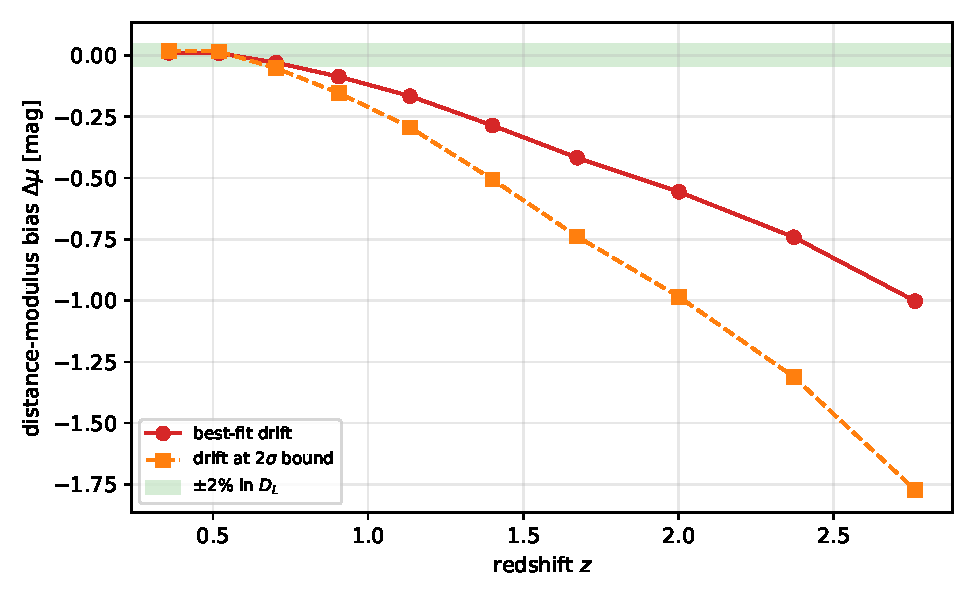
\includegraphics[width=\columnwidth]{fig5_bias}
\caption{Distance-modulus bias from using a constant slope when the slope drifts (Eq.~\ref{eq:bias}), for the best-fit $m$ and for its $2\sigma$ bound, against the $\pm2\%$ distance band.}
\label{fig:bias}
\end{figure}

Turning Eq.~\ref{eq:bias} around: a 2\% distance at $z=2$ ($\Delta\mu=0.043$\,mag) with $\Delta B=1.08$\,dex tolerates $\Delta\gamma=0.0066$, i.e.
\begin{equation}
\sigma_m\lesssim0.003 .
\end{equation}
The present catalogue delivers $\sigma_m=0.017$. Since $\sigma_m\propto N^{-1/2}$ at fixed scatter, reaching 0.003 needs $(0.017/0.003)^2\simeq30$ times more quasars of L20 quality, of order $6\times10^4$, or a reduction of the intrinsic scatter from 0.22 to $\lesssim0.06$\,dex \citep[the goal of][]{signorini24}, or, most realistically, an external distance anchor in every redshift shell so that $\gamma$ is never extrapolated across the lever arm. eROSITA \citep{sacchi25} and the \citet{risaliti26} sample are steps towards the first; none of the three is achieved yet. A flat $\gamma(z)$ measured to $\pm0.02$, which is what every current sample provides, is therefore a necessary but far from sufficient condition for a percent-level quasar $H_0$.

\section{Conclusions}
\begin{enumerate}\setlength{\itemsep}{1pt}
\item In the L20 catalogue, shell redshift and shell luminosity are collinear at $r=0.98$. A binned ``$\gamma(z)$ is flat'' test cannot distinguish redshift evolution from luminosity dependence ($\Delta{\mathrm{AIC}}=1.1$); the within-shell curvature, which is cosmology-free, can, and it excludes luminosity curvature as the origin of the observed drift at $3.7\sigma$.
\item A binning-free, cosmology-free joint likelihood gives $\gamma_0=0.582\pm0.011$, $\delta=0.225$\,dex, and $m=d\gamma/dz=-0.042^{+0.016}_{-0.017}$ (LR $p=0.007$; BIC neutral). Per-shell slope errors of 0.03--0.05 make $\sigma_m<0.013$ unattainable on this catalogue.
\item The drift survives truncation-corrected likelihoods, a photon-index term, distance detrending, and restriction to the homogeneous SDSS\,$\times$\,4XMM subsample, but not restriction to $z>0.7$, where $m=-0.022\pm0.019$. It is a low- versus high-redshift contrast, which reconciles the two sides of the literature on this catalogue.
\item The best-fit drift, if extrapolated with a single slope, biases quasar distances by 23\% at $z=2$; the $2\sigma$ bound allows 0.9\,mag. A 2\% quasar distance at $z=2$ requires $\sigma_m\simeq0.003$, thirty times the present statistics, or a distance anchor in every redshift shell.
\end{enumerate}

\section*{Reproducibility}
Every number in this paper is produced by the scripts \texttt{analysis3.py}--\texttt{analysis6.py} in the repository, from the unmodified VizieR file \texttt{data/lusso2020.tsv}; the JSON files in \texttt{results/} hold every quoted value. Total runtime is about 25 minutes on a laptop. Fitting used \textsc{scipy} and \textsc{emcee}. The analysis and drafting were assisted by Claude (Anthropic); no value in the text was typed by hand.

\begin{thebibliography}{99}\small
\bibitem[Avni \& Tananbaum(1986)]{avni86} Avni Y., Tananbaum H., 1986, ApJ, 305, 83
\bibitem[D'Agostini(2005)]{dagostini05} D'Agostini G., 2005, arXiv:physics/0511182
\bibitem[Dainotti et al.(2022)]{dainotti22} Dainotti M.~G., Bargiacchi G., Lenart A.~{\L}., Capozziello S., \'O Colg\'ain E., Solomon R., Stojkovic D., Sheikh-Jabbari M.~M., 2022, ApJ, 931, 106
\bibitem[Dainotti et al.(2023)]{dainotti23} Dainotti M.~G., Bargiacchi G., Lenart A.~{\L}., Nagataki S., Capozziello S., 2023, ApJ, 950, 45
\bibitem[Di Valentino et al.(2021)]{divalentino21} Di Valentino E., et al., 2021, Class. Quantum Grav., 38, 153001
\bibitem[Eddington(1913)]{eddington13} Eddington A.~S., 1913, MNRAS, 73, 359
\bibitem[Foreman-Mackey et al.(2013)]{foremanmackey13} Foreman-Mackey D., Hogg D.~W., Lang D., Goodman J., 2013, PASP, 125, 306
\bibitem[Gao et al.(2026)]{gao26} Gao J., Hu J., Chen Y., Zhao B., Xu L., 2026, arXiv:2606.27173
\bibitem[Haardt \& Maraschi(1991)]{haardt91} Haardt F., Maraschi L., 1991, ApJ, 380, L51
\bibitem[Kelly(2007)]{kelly07} Kelly B.~C., 2007, ApJ, 665, 1489
\bibitem[Khadka \& Ratra(2020)]{khadka20} Khadka N., Ratra B., 2020, MNRAS, 497, 263
\bibitem[Khadka \& Ratra(2021)]{khadka21} Khadka N., Ratra B., 2021, MNRAS, 502, 6140
\bibitem[Khadka \& Ratra(2022)]{khadka22} Khadka N., Ratra B., 2022, MNRAS, 510, 2753
\bibitem[Kubota \& Done(2018)]{kubota18} Kubota A., Done C., 2018, MNRAS, 480, 1247
\bibitem[Lenart et al.(2023)]{lenart23} Lenart A.~{\L}., Bargiacchi G., Dainotti M.~G., Nagataki S., Capozziello S., 2023, ApJS, 264, 46
\bibitem[Li et al.(2025)]{li25} Li X., Keeley R.~E., Shafieloo A., 2025, ApJ, 983, 141
\bibitem[Li et al.(2026)]{li26} Li G., Li Z., Song N., Chen C., Dong C., Tian J., Zhang Z., Li J., Tian H., Ma M., 2026, A\&A, 706, A337
\bibitem[Lusso \& Risaliti(2016)]{lusso16} Lusso E., Risaliti G., 2016, ApJ, 819, 154
\bibitem[Lusso \& Risaliti(2017)]{lusso17} Lusso E., Risaliti G., 2017, A\&A, 602, A79
\bibitem[Lusso et al.(2020)]{lusso20} Lusso E., et al., 2020, A\&A, 642, A150 (L20)
\bibitem[Lusso et al.(2025)]{lusso25} Lusso E., Risaliti G., Nardini E., 2025, A\&A, 697, A108
\bibitem[Petrosian et al.(2022)]{petrosian22} Petrosian V., Singal J., Mutchnick S., 2022, ApJ, 935, L19
\bibitem[Planck Collaboration(2020)]{planck20} Planck Collaboration, 2020, A\&A, 641, A6
\bibitem[Riess et al.(2022)]{riess22} Riess A.~G., et al., 2022, ApJ, 934, L7
\bibitem[Risaliti \& Lusso(2015)]{risaliti15} Risaliti G., Lusso E., 2015, ApJ, 815, 33
\bibitem[Risaliti \& Lusso(2019)]{risaliti19} Risaliti G., Lusso E., 2019, Nature Astron., 3, 272
\bibitem[Risaliti et al.(2026)]{risaliti26} Risaliti G., Lusso E., Nardini E., Niccolai C., Ralowski M., Sacchi A., Shlentsova A., Signorini M., Trefoloni B., 2026, arXiv:2606.07730
\bibitem[Sacchi et al.(2025)]{sacchi25} Sacchi A., Risaliti G., Signorini M., Nardini E., et al., 2025, A\&A, 703, A273
\bibitem[Signorini et al.(2024)]{signorini24} Signorini M., Risaliti G., Lusso E., Nardini E., et al., 2024, A\&A, 687, A32
\bibitem[Tananbaum et al.(1979)]{tananbaum79} Tananbaum H., et al., 1979, ApJ, 234, L9
\bibitem[Wang et al.(2022)]{wang22} Wang B., Liu Y., Yuan Z., Liang N., et al., 2022, ApJ, 940, 174
\bibitem[Wang et al.(2024)]{wang24} Wang B., Liu Y., Yu H., Wu P., 2024, ApJ, accepted, arXiv:2401.01540
\bibitem[Zaja\v{c}ek et al.(2024)]{zajacek24} Zaja\v{c}ek M., et al., 2024, ApJ, 961, 229
\end{thebibliography}
\end{document}
